\documentclass{beamer}
\usepackage{ctex, hyperref}
\usepackage{calligra}
\usepackage[T1]{fontenc}
\author{傅宇千}
\title{WHU Beamer Theme}
\subtitle{学术报告}
\institute{武汉大学电子信息学院}
\date{2020年4月6日}
\usepackage{WHU}

\begin{document}

\kaishu
\begin{frame}
	\titlepage
	\begin{figure}[htpb]
		\begin{center}
			
\includegraphics[width=0.2\linewidth]{pic/whulogo.eps}
		\end{center}
	\end{figure}
\end{frame}
\begin{frame}
\tableofcontents[sectionstyle=show,subsectionstyle=show/shaded/hide,subsubsectionstyle=show/shaded/hide]
\end{frame}


\section{课题背景}

\begin{frame}{用Beamer很高大上?}
\begin{itemize}
\item 大家都会\LaTeX{}
\item 好多学校都有自己的Beamer主题
\item 中文支持请选择 Xe\LaTeX{} 编译选项
\item 更好的公式支持性
\end{itemize}
\end{frame}

\section{研究现状}

\subsection{Beamer主题分类}

\begin{frame}
\begin{itemize}
\item 有一些 \LaTeX{} 自带的
\item 有一些Tsinghua的
\item WHU黄正华老师beamer主题
\item 本模板来源自 \newline \url{https://www.latexstudio.net/index/details/index/mid/215.html}
\item 最原始的Theme在这里:\cite{origin}(该链接已失效)
\end{itemize}
\end{frame}

\section{研究内容}

\subsection{美化主题}

\begin{frame}{这一份主题与原始的THU Beamer Theme区别在于}
\begin{itemize}
\item 目前只改了颜色和校徽
\item 原本的Theme做的很好了(我太菜了)	
\begin{figure}[htpb]
	\begin{center}
		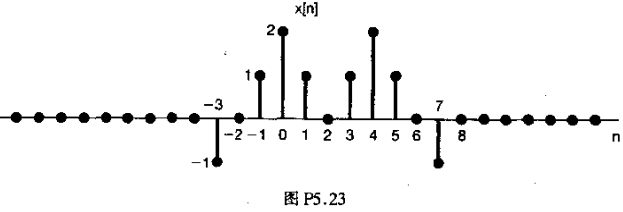
\includegraphics[width=0.9\linewidth]{pic/1.png}
	\end{center}
\end{figure}
\end{itemize}
\end{frame}

\section{计划进度}
\begin{frame}
	\begin{itemize}
\item 使用该Theme进行一些学术报告
\item 在使用过程中逐步进行Theme的修改
	\end{itemize}
\end{frame}

\section{参考文献}

\begin{frame}[allowframebreaks]
\bibliographystyle{alpha}
\bibliography{ref}
\end{frame}

\begin{frame}
\begin{center}
{\Huge Thanks!}
\end{center}
\end{frame}

\end{document}